% Full conference paper — 6 pages, 10 pt, double-column, IEEEtran
% Compile: pdflatex main && pdflatex main
%
\documentclass[10pt,conference]{IEEEtran}

\usepackage[T1]{fontenc}
\usepackage[utf8]{inputenc}
\usepackage{amsmath,amssymb}
\usepackage{booktabs}
\usepackage{url}
\usepackage{cite}
\usepackage{makecell}
\usepackage[table]{xcolor}
\usepackage{algorithm}
\usepackage{algpseudocode}
\usepackage{graphicx}
\usepackage{tikz}
\usetikzlibrary{arrows.meta,positioning}

\newcommand{\lmax}{L_{\max}}
\newcommand{\dmax}{\Delta_{\max}}
\newcommand{\umax}{U_{\max}}

% ─────────────────────────────────────────────────────────────────────────────
\title{\Large PhySDV: Physics-Grounded Data Generation and Risk-Aware\\
       Learned Task Offloading\\
       in Software-Defined Vehicles}

\author{%
  \IEEEauthorblockN{%
    Konstantinos Gyftodimos,\quad
    Eirini Liotou,\quad
    Kyriakos Chiotis,\quad
    George Dimitrakopoulos%
  }%
  \IEEEauthorblockA{%
    Dept.\ of Informatics and Telematics,
    Harokopio University of Athens (HUA), Athens, Greece\\
    \{kgyftodimos,\;eliotou,\;kchiotis,\;gdimitra\}@\textit{hua.gr}%
  }%
}

% ─────────────────────────────────────────────────────────────────────────────
\begin{document}
\maketitle

% ── Abstract ─────────────────────────────────────────────────────────────────
\begin{abstract}
Software-defined vehicles (SDVs) decouple automotive functions from fixed
electronic control units, turning perception into a schedulable service that
may execute on board, on a multi-access edge computing (MEC) server, or in
the cloud.  Selecting the execution tier per frame requires anticipating
network conditions that change on sub-second timescales, yet open,
\emph{labeled} datasets coupling vehicular radio state to offloading targets
remain scarce.  We present \textbf{PhySDV}, an open end-to-end framework
comprising (i)~a physics-grounded generative model (3GPP-calibrated path
loss, shadowing, Shannon-capacity throughput, queue-theoretic server
delay) emitting a 50\,000-sample labeled dataset across five road
archetypes; (ii)~a two-stage learned network-state predictor extended with
an upper-quantile variant for \emph{risk-aware} feasibility gating; and
(iii)~a QoS-constrained edge-first decision layer with hysteresis-based
stabilization.  We further introduce a three-level validation protocol
(structural, predictive, task-level): the generator's configured physics
are recoverable from the emitted data to within 1.6\%; a gradient-boosted
predictor attains 6.1\,ms MEC-RTT mean absolute error in a 1.3\,MB model;
and in closed loop the learned policy tracks a ground-truth oracle to
within QoS-neutral tier swaps (up to 98.8\% raw decision agreement).
Quantile gating raises worst-scenario latency-budget compliance from
94.0\% to 96.6\% at unchanged effective accuracy, while stabilization
suppresses 96\% of mode oscillations without delaying safety fallbacks.
Framework, dataset, and all experiments are released as open source.
\end{abstract}

\begin{IEEEkeywords}
software-defined vehicles, multi-access edge computing, computation
offloading, synthetic datasets, quality of service, quantile regression
\end{IEEEkeywords}

% ── I. Introduction ──────────────────────────────────────────────────────────
\section{Introduction}\label{sec:intro}

The software-defined vehicle (SDV) paradigm replaces dozens of
function-specific electronic control units with a zonal architecture built
around centralized, updatable high-performance computers, exposing
automotive functions as orchestrated services~\cite{liu2022sdv}.  This
shift makes workload placement a runtime software decision rather than a
wiring-harness decision: a perception service such as YOLOv8 object
detection~\cite{yolov8} may run on an on-board accelerator, be offloaded
to a road-side multi-access edge computing (MEC) server~\cite{etsi_mec},
or be shipped to a cloud data center---and the placement can be revised
continuously, even per camera frame.  Each tier trades accuracy against latency:
compact on-board models respond within milliseconds but lose accuracy,
whereas larger remote models are more accurate but pay a volatile network
round-trip time (RTT).  Advanced driving assistance imposes hard
quality-of-service (QoS) budgets---end-to-end latencies on the order of
100\,ms~\cite{3gpp22186}---so the tier decision must be re-evaluated
continuously as radio conditions evolve~\cite{liu2019autodriving}.

Making this decision \emph{predictively} requires estimating near-future
MEC and cloud RTT from observable vehicle and radio state.  Data-driven
network models~\cite{rusek2020routenet,almasan2022dtn} are natural
candidates but need labeled training data, and public vehicular datasets
coupling radio state to offloading-relevant targets (per-tier RTT,
utilization, reachability) are scarce: operator traces are proprietary,
while packet-level co-simulators~\cite{sommer2011veins,lopez2018sumo} do
not emit supervised-learning-ready labels and are heavyweight to configure
and run.

This paper closes that gap with \textbf{PhySDV}, an open, lightweight,
fully reproducible framework\footnote{\url{https://github.com/icsa-hua/PHYSDV}}
that spans the complete loop from radio physics to
per-frame offloading decisions.  Our contributions are:

\begin{enumerate}
  \item \textbf{A physics-grounded generative model and open dataset.}
        A 3GPP-calibrated log-distance channel~\cite{3gpp38901} with
        log-normal shadowing and stochastic non-line-of-sight (NLOS)
        excursions, composed with Shannon-capacity
        throughput~\cite{shannon1948}, per-user bandwidth sharing,
        queue-theoretic server delay~\cite{kleinrock}, and a diurnal load
        model.  The released dataset covers 50\,000 samples across five
        road archetypes with MEC inter-site distances from 300\,m to
        10\,km (Sec.~\ref{sec:datagen}).
  \item \textbf{A three-level validation protocol} for synthetic network
        datasets: \emph{structural} fidelity (the configured physics must
        be recoverable from the emitted data), \emph{predictive} fidelity
        (held-out error), and \emph{task-level} fidelity (closed-loop
        decision agreement against a ground-truth oracle)
        (Sec.~\ref{sec:validation}).
  \item \textbf{A deployable two-stage network-state predictor.}
        An availability classifier gates a multi-output RTT regressor,
        avoiding sentinel-value contamination.  A model-family study
        identifies gradient-boosted trees as the deployment choice:
        6.1\,ms MEC-RTT MAE in a 1.3\,MB model---700$\times$ smaller and
        3.8$\times$ faster than the random-forest baseline
        (Sec.~\ref{sec:predictor}).
  \item \textbf{Risk-aware QoS gating via quantile regression.}
        Feasibility is gated on the predicted \emph{upper quantile} (p90)
        of RTT rather than its conditional mean, converting symmetric
        prediction error into a one-sided safety margin and closing most
        of the latency-compliance gap to the oracle
        (Sec.~\ref{sec:policy}, \ref{sec:results}).
  \item \textbf{A stabilized, explainable decision layer.}  Edge-first
        feasibility selection with exponential smoothing and minimum-dwell
        hysteresis (safety bypass for infeasibility events) suppresses
        96\% of mode oscillations; every decision carries a
        machine-readable reason code, supporting the auditability that SDV
        safety cases require (Sec.~\ref{sec:policy}).
\end{enumerate}

All results are produced by seeded, single-command scripts shipped with
the framework.

% ── Figure 1: architecture ───────────────────────────────────────────────────
\begin{figure}[t]
\centering
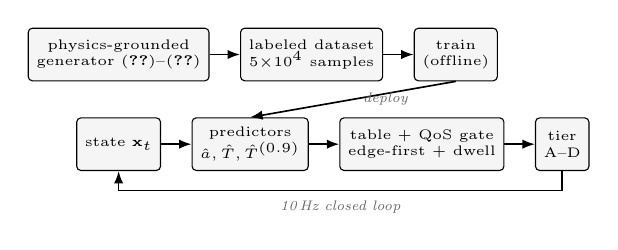
\begin{tikzpicture}[
  font=\tiny,
  box/.style={draw, rounded corners=1.5pt, align=center, inner sep=3pt,
              minimum height=19pt, fill=gray!8},
  lbl/.style={font=\tiny\itshape, text=black!60},
  arr/.style={-{Latex[length=4.5pt]}, semithick},
  node distance=13pt and 11pt
]
\node[box] (gen)  {physics-grounded\\generator \eqref{eq:pl}--\eqref{eq:tcloud}};
\node[box, right=of gen]  (data) {labeled dataset\\$5{\times}10^4$ samples};
\node[box, right=of data] (train) {train\\(offline)};
\node[box, below=of gen]  (state) {state $\mathbf{x}_t$};
\node[box, right=of state] (pred) {predictors\\$\hat a,\hat T,\hat T^{(0.9)}$};
\node[box, right=of pred]  (pol)  {table + QoS gate\\edge-first + dwell};
\node[box, right=of pol]   (mode) {tier\\A--D};
\draw[arr] (gen)   -- (data);
\draw[arr] (data)  -- (train);
\draw[arr] (train.south) -- node[lbl, right]{deploy} (pred.north);
\draw[arr] (state) -- (pred);
\draw[arr] (pred)  -- (pol);
\draw[arr] (pol)   -- (mode);
\draw[arr] (mode.south) -- +(0,-7pt) -|
  node[lbl, below, pos=0.25]{10\,Hz closed loop} (state.south);
\end{tikzpicture}
\caption{PhySDV architecture.  Offline: the generator emits labeled data
to train the predictors.  Online: per-frame estimates
($\hat a$, $\hat T$, $\hat T^{(0.9)}$) feed a QoS-gated, stabilized policy
that binds the SDV perception service to an execution tier.}
\label{fig:arch}
\end{figure}

% ── II. Related Work ─────────────────────────────────────────────────────────
\section{Related Work}\label{sec:related}

\textbf{Computation offloading.}  Offloading policy design is extensively
surveyed in~\cite{mao2017survey,mach2017survey}.  Learning-based policies
range from deep reinforcement learning over abstracted channel
models~\cite{chen2019offloading} to DNN partitioning between device and
cloud~\cite{kang2017neurosurgeon}.  These works
optimize the \emph{policy} while abstracting the network as a stationary or
coarsely-modeled resource; PhySDV is complementary: it supplies the missing
substrate---a reproducible, physically-consistent environment with labeled
network state---on which such policies can be trained and compared.

\textbf{Vehicular edge computing.}  Edge computing is a recognized enabler
for automotive perception~\cite{liu2019autodriving}, and the SDV
transition makes workload placement a first-class software
concern~\cite{liu2022sdv}.  Prior evaluations typically rely on
proprietary drive traces or on packet-level co-simulation stacks coupling
network and traffic simulators~\cite{sommer2011veins,lopez2018sumo}, which
reproduce protocol dynamics faithfully but require expert configuration,
run far slower than real time, and do not natively emit
supervised-learning labels.  PhySDV trades packet-level detail for an
analytically transparent link/queue model that generates labeled samples
in microseconds, is seeded end-to-end, and runs on a laptop.

\textbf{Learned network models and digital twins.}  RouteNet~\cite{rusek2020routenet}
and the network digital-twin agenda~\cite{almasan2022dtn} show that
learned surrogates predict network performance accurately---given training
data.  We operationalize this idea for the vehicular access segment and
add two missing elements: a validation protocol that checks the \emph{data
generator itself} (Sec.~\ref{sec:validation}), and a risk-aware quantile
formulation~\cite{koenker1978} that converts the surrogate's residual
uncertainty into a QoS safety margin.

% ── III. System Model ────────────────────────────────────────────────────────
\section{System Model and Problem Statement}\label{sec:model}

\subsection{Four-tier execution hierarchy}

We model perception as an SDV service: the vehicle streams camera frames
at rate $f$ (default 10\,Hz) to an object detector, and an on-board
orchestrator binds each frame $t$ to exactly one execution tier
$m \in \mathcal{M} = \{\mathrm{A}, \mathrm{B}, \mathrm{C}, \mathrm{D}\}$:
(A)~an on-board neural processing unit and (B)~the primary on-board GPU,
both running the compact YOLOv8n; (C)~a MEC server running YOLOv8m; and
(D)~a cloud data center running YOLOv8l (Table~\ref{tab:modes}).  Tier
profiles are configurable constants of the framework; shipped values use
published COCO~\cite{lin2014coco} mean average precision (mAP) figures for
YOLOv8~\cite{yolov8}, and a built-in benchmark module can substitute
latencies measured on real hardware.

\begin{table}[t]
\centering
\caption{Execution-tier profiles (as configured in the framework)}
\label{tab:modes}
\scriptsize\setlength{\tabcolsep}{4.5pt}
\begin{tabular}{@{}clrrrr@{}}
\toprule
\textbf{Tier} & \textbf{HW / model} & \textbf{Inf.\,(ms)} &
\textbf{Net.\,(ms)} & \textbf{mAP} & \textbf{$\Delta_m$} \\
\midrule
A & NPU / YOLOv8n   & 8 & 0            & 37.3 & 20.8\%$^{*}$ \\
B & GPU / YOLOv8n   & 5 & 0            & 37.3 & 20.8\%$^{*}$ \\
C & MEC / YOLOv8m   & 6 & $\hat T_C(t)$ & 50.2 &  4.9\%      \\
D & Cloud / YOLOv8l & 4 & $\hat T_D(t)$ & 52.9 &  0.0\%      \\
\bottomrule
\multicolumn{6}{@{}l}{$^{*}$Exceeds $\dmax=15\%$: activated only as emergency fallback.}
\end{tabular}
\end{table}

The \emph{accuracy loss} $\Delta_m$ of tier $m$ is defined against the
strongest model (YOLOv8l) over the safety-relevant road classes
$\mathcal{C}=\{\text{person, car, motorcycle, bus, truck}\}$:
\begin{equation}
\Delta_m \;=\; \frac{1}{|\mathcal{C}|} \sum_{c \in \mathcal{C}}
  \frac{\mathrm{AP}^{\mathrm{ref}}_{c} - \mathrm{AP}^{m}_{c}}
       {\mathrm{AP}^{\mathrm{ref}}_{c}},
\label{eq:accloss}
\end{equation}
using per-class average precision (AP).  Class-weighted evaluation matters:
the compact model's AP drop is far from uniform (28.1\% on
\emph{truck} vs.\ 15.7\% on \emph{person}), which a single aggregate mAP
delta would mask.

\subsection{QoS constraints and problem statement}

Let $T_m(t)$ denote the true end-to-end latency of tier $m$ at frame $t$
(inference plus network RTT; zero network term for A/B), $U_m(t)$ the
serving node's utilization, and $a(t)\in\{0,1\}$ MEC reachability.  The QoS
contract imposes three hard budgets: $\lmax = 100$\,ms end-to-end
latency~\cite{3gpp22186}, $\dmax = 15\%$ accuracy loss, and
$\umax = 95\%$ utilization.  The feasible set at frame $t$ is
\begin{align}
\mathcal{F}_t = \bigl\{\, m :\ &\rho_m(t)=1,\ T_m(t) \le \lmax, \nonumber\\[-1pt]
  &\Delta_m \le \dmax,\ U_m(t) < \umax \bigr\},
\label{eq:feasible}
\end{align}
where $\rho_m(t)$ is reachability ($\rho_C = a$, $\rho_m = 1$ otherwise).
The system must choose $m_t$ before executing frame $t$, i.e.\ using only
\emph{predictions} $\hat T_m(t), \hat U_m(t), \hat a(t)$ derived from the
observable state $\mathbf{x}_t$ (Sec.~\ref{sec:datagen}); mispredictions
that admit an infeasible tier translate directly into QoS violations.  This
motivates both the learned predictor (Sec.~\ref{sec:predictor}) and the
risk-aware gate (Sec.~\ref{sec:policy}).

% ── IV. Data generation ──────────────────────────────────────────────────────
\section{Physics-Grounded Data Generation}\label{sec:datagen}

Each sample couples a 13-dimensional observable state $\mathbf{x}$
(scenario class, vehicle speed, time of day, MEC distance, received signal
strength, channel bandwidth, cell load, connected users, handover flag,
payload size, wide-area-network (WAN) congestion, base cloud RTT, cloud
load) to five targets: MEC reachability $a$, MEC and cloud RTT, and MEC
and cloud utilization.  Targets are \emph{derived}, not sampled: every
label follows deterministically (up to bounded measurement noise) from the
physics below, which is what makes structural validation
(Sec.~\ref{sec:validation}) possible.

\subsection{Radio link}

Path loss follows a 3GPP-style log-distance model~\cite{3gpp38901} with
scenario-specific exponent $n$:
\begin{equation}
\mathrm{PL}(d) = 32.4 + 10\,n \log_{10} d + 20 \log_{10} f_c,
\label{eq:pl}
\end{equation}
with $d$ the MEC distance (m) and $f_c$ the carrier frequency (GHz).
Received signal strength adds log-normal shadowing and stochastic NLOS
excursions:
\begin{equation}
P_{\mathrm{rx}} = P_{\mathrm{tx}} + G - \mathrm{PL}(d) + X_\sigma
 - \mathbb{1}_{\mathrm{NLOS}}\,\mathcal{U}(25, 45)\ \text{dB},
\label{eq:rssi}
\end{equation}
where $X_\sigma \sim \mathcal{N}(0, \sigma^2)$ and NLOS occurs with
scenario probability $p_{\mathrm{NLOS}}$.  With orthogonal intra-cell
scheduling, the signal-to-interference-plus-noise ratio (SINR) is
\begin{equation}
\gamma = P_{\mathrm{rx}} - \bigl(-174 + 10\log_{10} B + N_F\bigr) - I_{\mathrm{ic}},
\label{eq:sinr}
\end{equation}
with bandwidth $B$ (Hz), noise figure $N_F = 7$\,dB, and a fixed
inter-cell interference margin $I_{\mathrm{ic}} = 5$\,dB.  MEC
reachability is the link-budget test $a = \mathbb{1}[\gamma > 0\,\text{dB}]$.

\subsection{Throughput and per-tier latency}

Spectral efficiency follows Shannon capacity~\cite{shannon1948} with an
implementation factor $\kappa = 0.6$ and a 256-QAM cap:
\begin{equation}
\eta_{\mathrm{se}} = \min\bigl(\kappa \log_2 (1 + 10^{\gamma/10}),\ 8.0\bigr)
\ \text{bit/s/Hz}.
\label{eq:se}
\end{equation}
The per-vehicle uplink rate shares the channel among $N_{\mathrm{UE}}$
users and degrades with server load $\rho_{\mathrm{mec}}$:
\begin{equation}
R = \eta_{\mathrm{se}} \cdot \tfrac{B}{N_{\mathrm{UE}}}
    \cdot (1 - 0.7\,\rho_{\mathrm{mec}}).
\label{eq:rate}
\end{equation}
MEC RTT composes upload, propagation, queueing, and handover terms:
\begin{equation}
T_{\mathrm{mec}} = \frac{8S}{R} + \frac{2d}{\nu}
 + \beta\,\rho_{\mathrm{mec}}^{2} + T_{\mathrm{ho}}\,\mathbb{1}_{\mathrm{ho}},
\label{eq:tmec}
\end{equation}
with payload $S$ (kB), propagation speed $\nu = 2\times10^{8}$\,m/s, a
queue-theoretic~\cite{kleinrock} load-quadratic delay ($\beta = 15$\,ms),
and $T_{\mathrm{ho}} = 20$\,ms per handover.  Cloud RTT adds a WAN model
with congestion index $g \in [0,1]$:
\begin{equation}
T_{\mathrm{cloud}} = T_{\mathrm{base}}
 + \frac{8S}{B_{\mathrm{wan}} / (1 + 3g)} + 30\,g .
\label{eq:tcloud}
\end{equation}
Both RTTs receive bounded multiplicative measurement noise
($\pm10\%$ MEC, $\pm5\%$ cloud).  Handover probability rises to 0.30 near
the cell edge at speed, cell load follows a Beta distribution scaled by a
1.5$\times$ diurnal rush-hour factor, and user count is Poisson with
scenario-specific mean---giving the dataset realistic temporal and spatial
correlation structure.

\subsection{Road-scenario parameterization}

Five archetypes (Table~\ref{tab:scenarios}) span two orders of magnitude in
MEC inter-site distance and the corresponding spectrum allocations, from a
dense 3.5\,GHz urban micro-cell layout to a 900\,MHz rural macro cell.

\begin{table}[t]
\centering
\caption{Road-scenario profiles}
\label{tab:scenarios}
\scriptsize\setlength{\tabcolsep}{3.6pt}
\begin{tabular}{@{}lrrrrrr@{}}
\toprule
\textbf{Scenario} & \textbf{ISD} & \textbf{Speed} & $f_c$ & $B$ &
$n$ & $\bar N_{\mathrm{UE}}$ \\
 & (m) & (km/h) & (GHz) & (MHz) & & \\
\midrule
urban\_dense  &    300 & 20--50   & 3.5 & 100 & 3.5 & 40 \\
urban\_sparse &    800 & 30--70   & 3.5 & 100 & 3.0 & 20 \\
suburban      &  2\,000 & 50--90  & 2.1 &  40 & 2.6 & 10 \\
highway       &  5\,000 & 80--130 & 2.1 &  20 & 2.2 &  5 \\
rural         & 10\,000 & 60--100 & 0.9 &  10 & 2.0 &  2 \\
\bottomrule
\end{tabular}
\end{table}

% ── V. Predictor ─────────────────────────────────────────────────────────────
\section{Learned Network-State Predictor}\label{sec:predictor}

\subsection{Two-stage formulation}

Unreachable frames have no finite MEC RTT; encoding them with a sentinel
value corrupts regression training, while discarding them biases the
classifier.  PhySDV therefore factorizes the predictor:
a binary classifier estimates $\hat a(t)$, and a multi-output regressor
estimates RTT and utilization; at inference time the regressor's MEC
output is masked whenever $\hat a = 0$.  Both stages share one
preprocessing pipeline: one-hot scenario encoding, standardization, and a
cyclic encoding of the time of day,
$(\sin, \cos)(2\pi h / 24)$, which removes the artificial midnight
discontinuity.  Utilization targets are near-pass-through in the current
generator (the serving node reports its own load in-band) and are retained
for schema completeness; the substantive learning problem is RTT
prediction, on which we focus.

\subsection{Model-family study}

Deployment constraints---model size, single-frame
latency, retraining cost---matter as much as accuracy on an automotive
platform.  We compare five families under identical preprocessing and an
80/20 split, all implemented in scikit-learn~\cite{pedregosa2011sklearn}
(Table~\ref{tab:predictors}).  MEC-RTT metrics are computed
\emph{only on reachable test rows}, the operationally meaningful regime.
A linear model fails outright on MEC RTT (R\textsuperscript{2} $<0$): the
target is dominated by the nonlinear interaction of link budget, bandwidth
share, and load.  Bagged trees (the framework's original default) model
MEC RTT well but regress the smooth WAN target poorly and serialize to
926\,MB.  Histogram gradient boosting~\cite{friedman2001} dominates on
both targets simultaneously---6.12\,ms MEC MAE, 1.69\,ms cloud MAE---in a
1.3\,MB artifact with 3.8\,ms single-frame latency, and is therefore the
recommended deployment predictor.  The availability stage is
near-perfect for every family (gradient boosting: 100.0\% test accuracy),
as expected: the label is a deterministic link-budget threshold
(Sec.~\ref{sec:datagen}), and this result should be read as a consistency
check, not a claim of difficulty.

\begin{table}[t]
\centering
\caption{Predictor comparison (80/20 split; MEC RTT scored on reachable
rows). $\dagger$\,=\,framework default; bold\,=\,recommended.}
\label{tab:predictors}
\scriptsize\setlength{\tabcolsep}{3.2pt}
\begin{tabular}{@{}lrrrrrr@{}}
\toprule
 & \multicolumn{2}{c}{\textbf{MEC RTT}} & \multicolumn{2}{c}{\textbf{Cloud RTT}} & & \\
\cmidrule(lr){2-3}\cmidrule(lr){4-5}
\textbf{Model} & MAE & R\textsuperscript{2} & MAE & R\textsuperscript{2} &
\textbf{Lat.\,(ms)} & \textbf{Size} \\
\midrule
Ridge (linear)      & 122.8 & $-2.62$ & 1.67 & 0.975 &  1.1 & 3\,kB \\
Random forest$^\dagger$~\cite{breiman2001} & 10.5 & 0.930 & 4.06 & 0.810 & 14.3 & 926\,MB \\
Extra trees         &  8.1 & 0.940 & 4.29 & 0.794 & 14.1 & 1.43\,GB \\
\textbf{Hist.\ grad.\ boosting} & \textbf{6.1} & \textbf{0.959} & \textbf{1.69} & \textbf{0.974} & \textbf{3.8} & \textbf{1.3\,MB} \\
MLP (128--64)       &  7.1 & 0.952 & 1.80 & 0.970 &  1.3 & 0.3\,MB \\
\bottomrule
\end{tabular}
\end{table}

Impurity-based attribution on the tree ensembles confirms the physics:
received signal strength dominates (91\% of split gain), followed by
channel bandwidth, user count, and scenario class---mirroring the causal
chain of \eqref{eq:pl}--\eqref{eq:tmec}.

\subsection{Risk-aware quantile variant}

A point predictor minimizing squared error is calibrated to the
conditional mean, so roughly half of its errors are underestimates; each
underestimate near the budget boundary can admit a tier whose \emph{true}
latency violates $\lmax$.  We therefore train upper-quantile RTT
regressors with pinball loss~\cite{koenker1978} at $\alpha = 0.9$
(gradient boosting, MEC model fitted on reachable rows only); held-out
coverage is 88.5\% (MEC) and 88.1\% (cloud) against the 90\% target.  The
decision layer can then gate feasibility on $\hat T^{(\alpha)}_m$ instead
of $\hat T_m$---a one-line policy change that turns residual model
uncertainty into a one-sided safety margin.

% ── VI. Decision layer ───────────────────────────────────────────────────────
\section{QoS-Aware Decision Layer}\label{sec:policy}

Algorithm~\ref{alg:loop} summarizes the per-frame loop.  Predictions are
smoothed by an exponential moving average (EMA, $\alpha_s = 0.3$) to damp
frame-to-frame jitter.  The feasibility gate applies
\eqref{eq:feasible} with either the mean or the quantile RTT estimate.
Among feasible tiers the policy is \emph{edge-first}: the MEC tier is
preferred over cloud unless the cloud model offers more than
$\delta = 5$ mAP points of improvement, conserving WAN bandwidth; if no
tier is feasible (e.g.\ a connectivity outage), the loop falls back to the
on-board GPU with an explicit reason code.  Every decision emits such a
code (\texttt{edge\_first\_within\_map\_delta},
\texttt{fallback\_no\_feasible\_mode}, \ldots), giving SDV integrators an
audit trail for each frame.

Because the feasibility boundary can sit between two near-equivalent
tiers, raw per-frame decisions oscillate.  A minimum-dwell hysteresis
filter commits a switch only after the new tier persists for $k$
consecutive frames ($k = 5$); infeasibility-triggered fallbacks
\emph{bypass} the filter, so safety-critical transitions are never
delayed.  Sec.~\ref{sec:results} quantifies the resulting
stability--responsiveness trade-off.

\begin{algorithm}[t]
\caption{PhySDV per-frame offloading decision}
\label{alg:loop}
\begin{algorithmic}[1]
\State observe state $\mathbf{x}_t$; predict $\hat a$, $\hat T_C$, $\hat T_D$
       (optionally $\hat T^{(\alpha)}_C$, $\hat T^{(\alpha)}_D$), $\hat U_C$, $\hat U_D$
\State $\tilde T_m \gets \alpha_s \hat T_m + (1-\alpha_s)\,\tilde T_m$
       \Comment{EMA; reset on $\hat a = 0$}
\State build table: tiers A/B static; C/D $\gets (\tilde T_m, \hat U_m)$
\State $\mathcal{F}_t \gets$ feasibility gate \eqref{eq:feasible}
\If{$\mathcal{F}_t = \emptyset$}
    \State $m_t \gets$ B; \textbf{reason} $\gets$ \texttt{fallback}; force switch
\ElsIf{$\{C, D\} \subseteq \mathcal{F}_t$ and
       $\mathrm{mAP}_D - \mathrm{mAP}_C < \delta$}
    \State $m_t \gets$ C \Comment{edge-first}
\Else
    \State $m_t \gets \arg\max_{m \in \mathcal{F}_t} \mathrm{mAP}_m$
\EndIf
\State $m_t \gets \mathrm{Dwell}_k(m_t)$ \Comment{hysteresis; bypassed on force}
\end{algorithmic}
\end{algorithm}

% ── VII. Validation methodology ──────────────────────────────────────────────
\section{Three-Level Validation Protocol}\label{sec:validation}

Synthetic datasets are only useful if their fidelity is testable.  We
validate PhySDV at three levels, each with a falsifiable criterion:

\textbf{V1 --- Structural fidelity.}  The generator's configured physics
must be \emph{recoverable} from the emitted data by an independent
estimator.  We re-fit the path-loss model \eqref{eq:pl} to the generated
(distance, signal-strength) pairs per scenario using iteratively
re-weighted least squares (sigma-clipping strips the NLOS mixture), and
compare recovered exponents and residual spreads to the configuration.

\textbf{V2 --- Predictive fidelity.}  Standard held-out metrics
(Table~\ref{tab:predictors}), with the sentinel-aware protocol of
Sec.~\ref{sec:predictor} and quantile-coverage calibration.

\textbf{V3 --- Task-level fidelity.}  Metrics V1--V2 do not establish
that predictions are good enough \emph{for the decisions they drive}.  We
therefore replay the closed loop against ground truth: the simulator's
deterministic physics yield the true $T_m(t), a(t)$ per frame, an
\emph{oracle} policy decides with these true values, and the learned
policy is scored on (i)~decision agreement with the oracle, (ii)~true
latency-budget compliance, and (iii)~effective detection quality.  We
propose V3---rarely reported in offloading studies---as the primary
acceptance criterion for learned offloading stacks.

% ── VIII. Results ────────────────────────────────────────────────────────────
\section{Experimental Results}\label{sec:results}

All experiments run CPU-only (Intel Core Ultra~9 275HX, 24 threads,
64\,GB RAM), fixed seed 42, on the released 50\,000-sample dataset;
closed-loop runs simulate 1\,000 frames per scenario at 10\,Hz.

\subsection{V1: structural fidelity}

Table~\ref{tab:physics} shows the recovered path-loss exponents within
0.1--1.6\% of their configured values, with clipped residual spread
tracking the configured shadowing $\sigma$.  The diurnal model is likewise
recovered: mean cell load is 42.6\% in rush hours vs.\ 28.6\%
off-peak---a 1.49$\times$ ratio against the configured 1.5$\times$.
Emergent per-scenario structure (Table~\ref{tab:dataset}) is physically
plausible: availability falls with NLOS-rich dense deployments, and MEC
RTT worsens as user density grows.

\begin{table}[t]
\centering
\caption{V1: recovery of configured physics from the emitted data}
\label{tab:physics}
\scriptsize\setlength{\tabcolsep}{4.2pt}
\begin{tabular}{@{}lcccc@{}}
\toprule
\textbf{Scenario} & $n$ (conf.) & $n$ (recov.) & $\sigma$ (conf.) & resid.\ (dB) \\
\midrule
urban\_dense  & 3.5 & 3.44 & 8 & 8.00 \\
urban\_sparse & 3.0 & 2.99 & 8 & 7.35 \\
suburban      & 2.6 & 2.61 & 6 & 5.18 \\
highway       & 2.2 & 2.19 & 4 & 3.35 \\
rural         & 2.0 & 2.00 & 4 & 3.49 \\
\bottomrule
\end{tabular}
\end{table}

\begin{table}[t]
\centering
\caption{Per-scenario dataset statistics.  ``C$<$D'' = share of reachable
samples where MEC RTT beats cloud RTT.}
\label{tab:dataset}
\scriptsize\setlength{\tabcolsep}{3.4pt}
\begin{tabular}{@{}lrrrrr@{}}
\toprule
\textbf{Scenario} & \textbf{Avail.} & \makecell{\textbf{MEC RTT}\\med.\,/\,p95 (ms)} &
\makecell{\textbf{Cloud RTT}\\med.\,/\,p95 (ms)} & \textbf{C$<$D} \\
\midrule
urban\_dense  & 80.8\% & 78.7 / 319.3 & 59.0 / 73.2  & 33.0\% \\
urban\_sparse & 83.2\% & 41.7 / 158.3 & 64.2 / 81.6  & 70.9\% \\
suburban      & 91.4\% & 39.3 / 128.2 & 69.7 / 87.2  & 80.9\% \\
highway       & 95.9\% & 34.0 / 110.3 & 72.4 / 92.2  & 86.9\% \\
rural         & 98.7\% & 29.3 / 133.1 & 81.0 / 103.0 & 88.7\% \\
\bottomrule
\end{tabular}
\end{table}

A key emergent effect deserves emphasis: in the dense-urban archetype the
\emph{edge is not the faster tier}---MEC RTT beats cloud RTT in only 33\%
of reachable samples, because 40 users share the cell and the
$n = 3.5$ path loss erodes per-user throughput, while p95 MEC RTT
(319\,ms) exceeds the latency budget outright.  Static ``edge
always wins'' assumptions embedded in many offloading heuristics fail
exactly where traffic is densest; per-frame prediction is not an
optimization but a requirement.

\subsection{V2: predictive fidelity}

Table~\ref{tab:predictors} (discussed in Sec.~\ref{sec:predictor})
summarizes held-out accuracy, latency, and footprint;
the recommended gradient-boosted predictor reaches 6.1\,ms MEC-RTT MAE
(R\textsuperscript{2} = 0.959 on reachable rows) and 1.69\,ms cloud MAE,
with quantile heads calibrated to within 1.9~points of nominal coverage.

\subsection{V3: closed-loop, task-level fidelity}

Table~\ref{tab:closedloop} compares policies over all five scenarios
(5\,000 decisions per policy).  Static baselines expose the trade-off
space: \emph{Always-B} meets latency trivially but violates the accuracy
budget on every frame; \emph{Always-D} is accurate but consumes WAN
uplink on 100\% of frames with 73.5\,ms mean latency and drops to 96.6\%
compliance in the rural archetype; \emph{Always-C} collapses to 53.5\%
latency compliance in dense urban (mean true latency 120.5\,ms).  The
learned policy tracks the oracle closely: mean-gated PhySDV achieves
96.9\% compliance and identical effective mAP (50.6) to the oracle while
touching the WAN on only 14.6\% of frames.

\begin{table}[t]
\centering
\caption{V3: closed-loop policy comparison, mean over five scenarios
(5\,000 frames).  Lat.\,/\,Acc.\,=\,latency\,/\,accuracy-budget
compliance; $\overline{T}$\,=\,mean true latency; WAN\,=\,cloud share;
Sw.\,=\,switches per 1\,000 frames.}
\label{tab:closedloop}
\scriptsize\setlength{\tabcolsep}{3.0pt}
\begin{tabular}{@{}lrrrrrr@{}}
\toprule
\textbf{Policy} & \textbf{Lat.} & \textbf{Acc.} & \textbf{mAP} &
$\overline{T}$ (ms) & \textbf{WAN} & \textbf{Sw.} \\
\midrule
Always-B (on-board)   & 100.0\% & 0.0\%   & 37.3 &  5.0 & 0\%    & 0 \\
Always-C (MEC)        & 86.4\%  & 100\% & 50.2 & 64.1 & 0\%    & 0 \\
Always-D (cloud)      & 99.3\%  & 100\% & 52.9 & 73.5 & 100\%  & 0 \\
\midrule
PhySDV, no EMA        & 99.5\%  & 100\% & 50.6 & 50.5 & 14.0\% & 142 \\
PhySDV (EMA)          & 96.9\%  & 100\% & 50.6 & 51.8 & 14.6\% & 47 \\
PhySDV q90 (EMA)      & 97.9\%  & 100\% & 50.7 & 51.0 & 17.9\% & 43 \\
PhySDV q90 + dwell    & 96.3\%  & 100\% & 50.7 & 52.8 & 18.2\% & 6 \\
\midrule
Oracle (true state)   & 100.0\% & 100\% & 50.6 & 50.6 & 13.7\% & 139 \\
\bottomrule
\end{tabular}
\end{table}

\textbf{Oracle agreement.}  Per-frame decision agreement between
mean-gated PhySDV and the oracle is 98.5--98.8\% in the suburban, highway,
and rural archetypes, 89.7\% in sparse urban, and 78.6\% in dense
urban---precisely where Table~\ref{tab:dataset} shows MEC and cloud in a
near-tie.  These disagreements are QoS-neutral swaps within the feasible
set: dense-urban effective mAP (51.7 vs.\ 51.5) and mean latency (69.2
vs.\ 67.7\,ms) stay within 3\% of the oracle.

\textbf{Risk-aware gating.}  Mean-gating leaves a compliance gap to the
oracle concentrated in the two urban archetypes (94.6\% and 94.0\%),
exactly where prediction error meets a tight feasibility boundary.
Switching the gate to the calibrated p90 estimate closes most of it
(Fig.~\ref{fig:gating}): dense-urban compliance rises from 94.6\% to
97.0\% and sparse-urban from 94.0\% to 96.6\%, lifting the five-scenario
mean from 96.9\% to 97.9\%.  Notably, effective accuracy is
\emph{unchanged} (mAP 50.7): the conservatism is priced in WAN share,
which rises 3.3 points to 17.9\% as borderline MEC frames divert to the
cloud---making the quantile level $\alpha$ an explicit, per-deployment
dial trading WAN budget for latency assurance.

\begin{figure}[t]
\centering
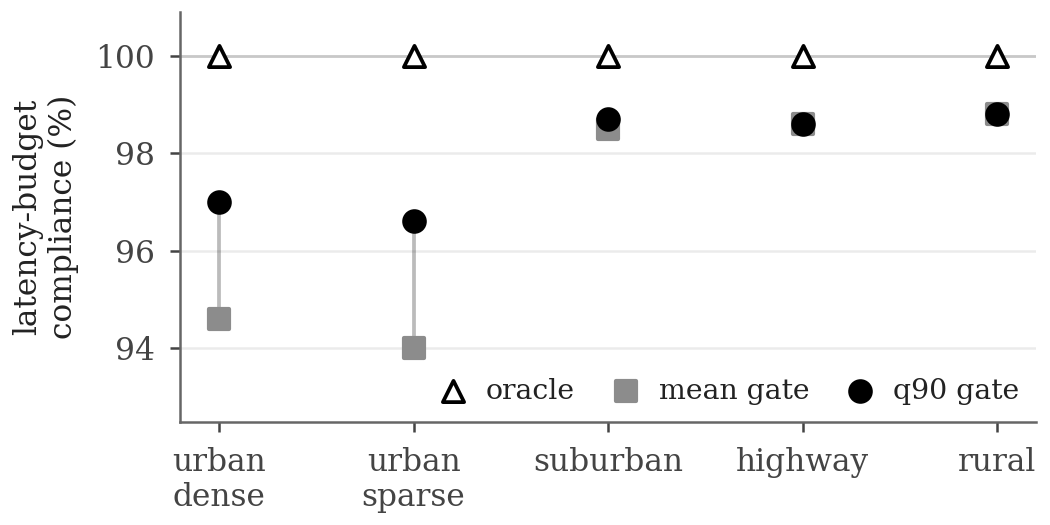
\includegraphics[width=0.92\columnwidth]{figures/compliance_gating.png}
\caption{V3 latency-budget compliance per scenario: gating feasibility on
the calibrated p90 RTT estimate (q90) recovers most of the gap between
mean-gated decisions and the ground-truth oracle, concentrated in the two
urban archetypes.}
\label{fig:gating}
\end{figure}

\textbf{Stability.}  Raw per-frame decisions switch 142 times per 1\,000
frames; EMA smoothing cuts this to 47; adding the dwell filter yields
6 switches ($-$96\% vs.\ raw) while mean latency compliance changes by
only 1.6 points (97.9\% $\to$ 96.3\%).  For an SDV integrator each
switch is a service reconfiguration (stream redirection, codec and
session renegotiation), so this two-order-of-magnitude reduction is an
enabler in itself.  Because infeasibility events bypass the filter, the
injected outage below is still handled instantly.

\textbf{Outage failover.}  Fig.~\ref{fig:outage} replays a dense-urban run
with a 3\,s connectivity outage injected at frame 80 (MEC unreachable,
cloud RTT inflated to 200\,ms).  Both raw and stabilized policies fall
back to the on-board GPU \emph{on the frame of outage onset} (zero-frame
delay)---accepting the temporary accuracy-budget violation, which is
exactly the intended emergency semantics.  The raw trace restores MEC
service on the first post-outage frame; the stabilized trace holds the
fallback for $k{-}1=4$ extra frames (0.4\,s), a conservative re-entry
that avoids flapping if connectivity is still unstable.

\begin{figure}[t]
\centering
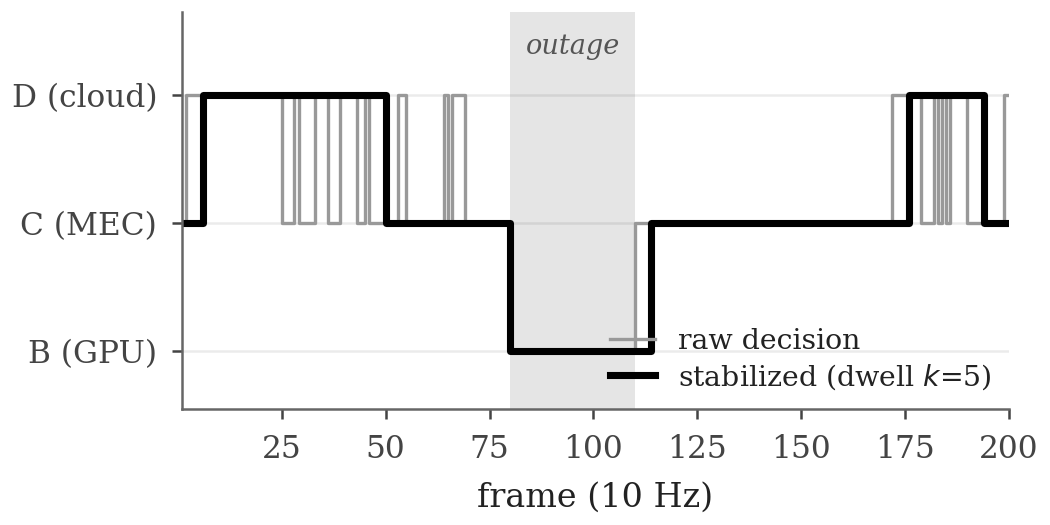
\includegraphics[width=0.92\columnwidth]{figures/outage_timeline.png}
\caption{Outage failover, dense urban, q90-gated policy.  A simulated
outage (frames 80--109, shaded) makes MEC unreachable and inflates cloud
RTT beyond the budget.  Fallback to the on-board tier is immediate in both
traces because infeasibility bypasses the dwell filter; the stabilized
trace additionally suppresses the C/D chatter and holds the fallback for
$k{-}1 = 4$ extra frames (0.4\,s) after the outage clears.}
\label{fig:outage}
\end{figure}

\textbf{Runtime.}  The full control loop---feature assembly, availability
classification, mean and quantile RTT prediction, table update, gating,
and stabilization---runs in 10.8\,ms median per frame with the
recommended predictor (6.2\,ms without the quantile heads; 27.9\,ms with
the random-forest default), comfortably inside a 10\,Hz budget on CPU
only.  Dataset generation and full training complete in under a minute
combined, with no GPU, testbed, or network connection required.

\subsection{Discussion and limitations}

\textbf{Synthetic-to-real gap.}  PhySDV's labels are internally
consistent by construction, and V1 shows they faithfully encode the
configured physics---but the configuration itself abstracts reality: a
single serving cell, no packet-level protocol effects, no multi-vehicle
decision coupling, and utilization targets that the current generator
exposes as observable telemetry.  The intended workflow is
\emph{calibration}: every constant in \eqref{eq:pl}--\eqref{eq:tcloud} is
a named configuration parameter re-fittable from drive tests, and the
benchmark module replaces configured tier latencies with measured ones;
the validation protocol then re-runs unchanged.

\textbf{Availability triviality.}  MEC reachability is a deterministic
link-budget function in the generator, so near-perfect classification is
expected; real-world reachability (RRC state, admission control) is
noisier.  The two-stage architecture is agnostic to this---only the
classifier's operating point would change.

\textbf{Scope of the policy.}  The decision layer is deliberately a
transparent, auditable baseline (feasibility gate + lexicographic
preference); its value here is that the framework makes \emph{any} policy
comparable under V3.  Plugging DRL policies~\cite{chen2019offloading} into
the same loop is direct future work, as are multi-vehicle contention and
trace-driven calibration against public 5G drive tests.

% ── IX. Conclusion ───────────────────────────────────────────────────────────
\section{Conclusion}\label{sec:conclusion}

PhySDV contributes an open, physics-grounded substrate for studying
QoS-constrained perception offloading in software-defined vehicles: a
labeled 50\,k-sample dataset whose generating physics are recoverable from
the data itself, a deployable two-stage predictor in automotive footprint
(1.3\,MB, 3.8\,ms), a risk-aware quantile gate that converts prediction
uncertainty into QoS safety margin, and a stabilized, explainable decision
layer---validated by a three-level protocol culminating in closed-loop
oracle agreement of up to 98.8\%.  Every number in this paper regenerates
from a seeded script on a laptop.  We offer PhySDV as a common, extensible
baseline on which offloading policies, predictors, and calibrated
deployment profiles can be compared under identical, falsifiable
conditions.

% ── Acknowledgment ───────────────────────────────────────────────────────────
\section*{Acknowledgment}

This work has been funded by the Shift2SDV project (Grant Agreement
No.~101194245), supported by the Chips Joint Undertaking and its members,
including top-up funding by the national authorities of Austria, Denmark,
Germany, Greece, Finland, Italy, Netherlands, Poland, Portugal, Spain, and
Turkey.

% ── References ───────────────────────────────────────────────────────────────
\begin{thebibliography}{21}

\bibitem{liu2022sdv}
Z.~Liu, W.~Zhang, and F.~Zhao,
``Impact, challenges and prospect of software-defined vehicles,''
\textit{Automotive Innovation}, vol.~5, pp.~180--194, 2022.

\bibitem{yolov8}
G.~Jocher, A.~Chaurasia, and J.~Qiu,
``Ultralytics YOLOv8,'' GitHub, 2023.
[Online]. Available: \url{https://github.com/ultralytics/ultralytics}

\bibitem{etsi_mec}
ETSI,
``GS MEC~003: MEC framework and reference architecture, v3.1.1,'' 2022.

\bibitem{3gpp22186}
3GPP,
``TS~22.186: Enhancement of 3GPP support for V2X scenarios, v16.2.0,''
3rd Generation Partnership Project, 2019.

\bibitem{liu2019autodriving}
S.~Liu, L.~Liu, J.~Tang, B.~Yu, Y.~Wang, and W.~Shi,
``Edge computing for autonomous driving: Opportunities and challenges,''
\textit{Proc. IEEE}, vol.~107, no.~8, pp.~1697--1716, 2019.

\bibitem{rusek2020routenet}
K.~Rusek, J.~Su\'arez-Varela, P.~Almasan, P.~Barlet-Ros, and
A.~Cabellos-Aparicio,
``RouteNet: Leveraging graph neural networks for network modeling and
optimization in SDN,''
\textit{IEEE J. Sel. Areas Commun.}, vol.~38, no.~10, pp.~2260--2270, 2020.

\bibitem{almasan2022dtn}
P.~Almasan \textit{et~al.},
``Network digital twin: Context, enabling technologies, and opportunities,''
\textit{IEEE Commun. Mag.}, vol.~60, no.~11, pp.~22--27, 2022.

\bibitem{sommer2011veins}
C.~Sommer, R.~German, and F.~Dressler,
``Bidirectionally coupled network and road traffic simulation for improved
IVC analysis,''
\textit{IEEE Trans. Mobile Comput.}, vol.~10, no.~1, pp.~3--15, 2011.

\bibitem{lopez2018sumo}
P.~A. Lopez \textit{et~al.},
``Microscopic traffic simulation using SUMO,''
in \textit{Proc. IEEE Int. Conf. Intelligent Transportation Systems
(ITSC)}, 2018, pp.~2575--2582.

\bibitem{3gpp38901}
3GPP,
``TR~38.901: Study on channel model for frequencies from 0.5 to 100~GHz,
v16.1.0,'' 3rd Generation Partnership Project, 2019.

\bibitem{shannon1948}
C.~E. Shannon,
``A mathematical theory of communication,''
\textit{Bell Syst. Tech. J.}, vol.~27, pp.~379--423, 1948.

\bibitem{kleinrock}
L.~Kleinrock,
\textit{Queueing Systems, Volume 1: Theory}.
New York, NY, USA: Wiley, 1975.

\bibitem{mao2017survey}
Y.~Mao, C.~You, J.~Zhang, K.~Huang, and K.~B. Letaief,
``A survey on mobile edge computing: The communication perspective,''
\textit{IEEE Commun. Surveys Tuts.}, vol.~19, no.~4, pp.~2322--2358, 2017.

\bibitem{mach2017survey}
P.~Mach and Z.~Becvar,
``Mobile edge computing: A survey on architecture and computation
offloading,''
\textit{IEEE Commun. Surveys Tuts.}, vol.~19, no.~3, pp.~1628--1656, 2017.

\bibitem{chen2019offloading}
X.~Chen, H.~Zhang, C.~Wu, S.~Mao, Y.~Ji, and M.~Bennis,
``Optimized computation offloading performance in virtual edge computing
systems via deep reinforcement learning,''
\textit{IEEE Internet Things J.}, vol.~6, no.~3, pp.~4005--4018, 2019.

\bibitem{kang2017neurosurgeon}
Y.~Kang \textit{et~al.},
``Neurosurgeon: Collaborative intelligence between the cloud and mobile
edge,''
in \textit{Proc. ACM ASPLOS}, 2017, pp.~615--629.

\bibitem{lin2014coco}
T.-Y. Lin \textit{et~al.},
``Microsoft COCO: Common objects in context,''
in \textit{Proc. Eur. Conf. Computer Vision (ECCV)}, 2014, pp.~740--755.

\bibitem{breiman2001}
L.~Breiman,
``Random forests,''
\textit{Machine Learning}, vol.~45, no.~1, pp.~5--32, 2001.

\bibitem{friedman2001}
J.~H. Friedman,
``Greedy function approximation: A gradient boosting machine,''
\textit{Ann. Statist.}, vol.~29, no.~5, pp.~1189--1232, 2001.

\bibitem{koenker1978}
R.~Koenker and G.~Bassett,
``Regression quantiles,''
\textit{Econometrica}, vol.~46, no.~1, pp.~33--50, 1978.

\bibitem{pedregosa2011sklearn}
F.~Pedregosa \textit{et~al.},
``Scikit-learn: Machine learning in Python,''
\textit{J. Mach. Learn. Res.}, vol.~12, pp.~2825--2830, 2011.

\end{thebibliography}

\end{document}
